\subsection{Forward proton efficiency} \label{sec:FC_eff}

\begin{figure}[htbp]
  \centering
  \begin{tabular}{cc}
    \begin{minipage}{0.5\hsize}
      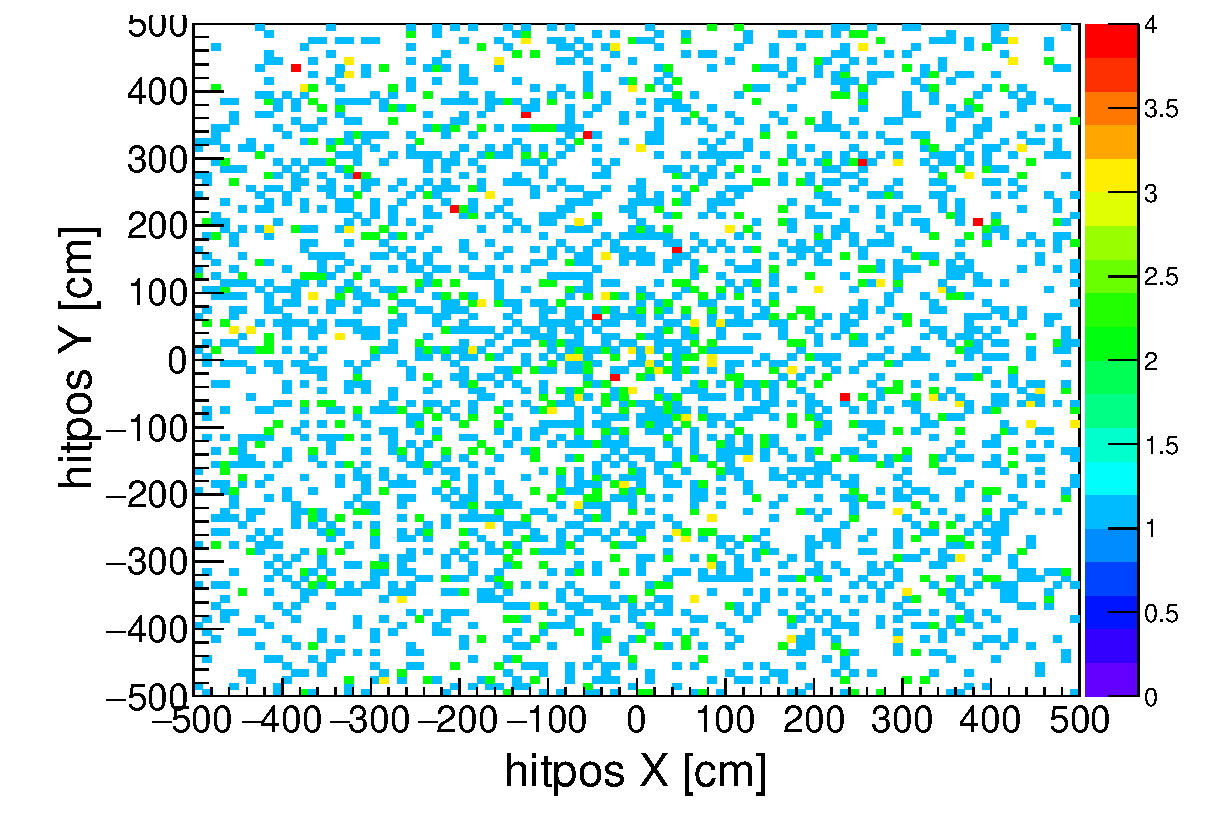
\includegraphics[width=5cm]{../pic/Run78/CDS_Lpim//kp_hitpos_Lpim_p.eps}
    \end{minipage}

    \begin{minipage}{0.5\hsize}
      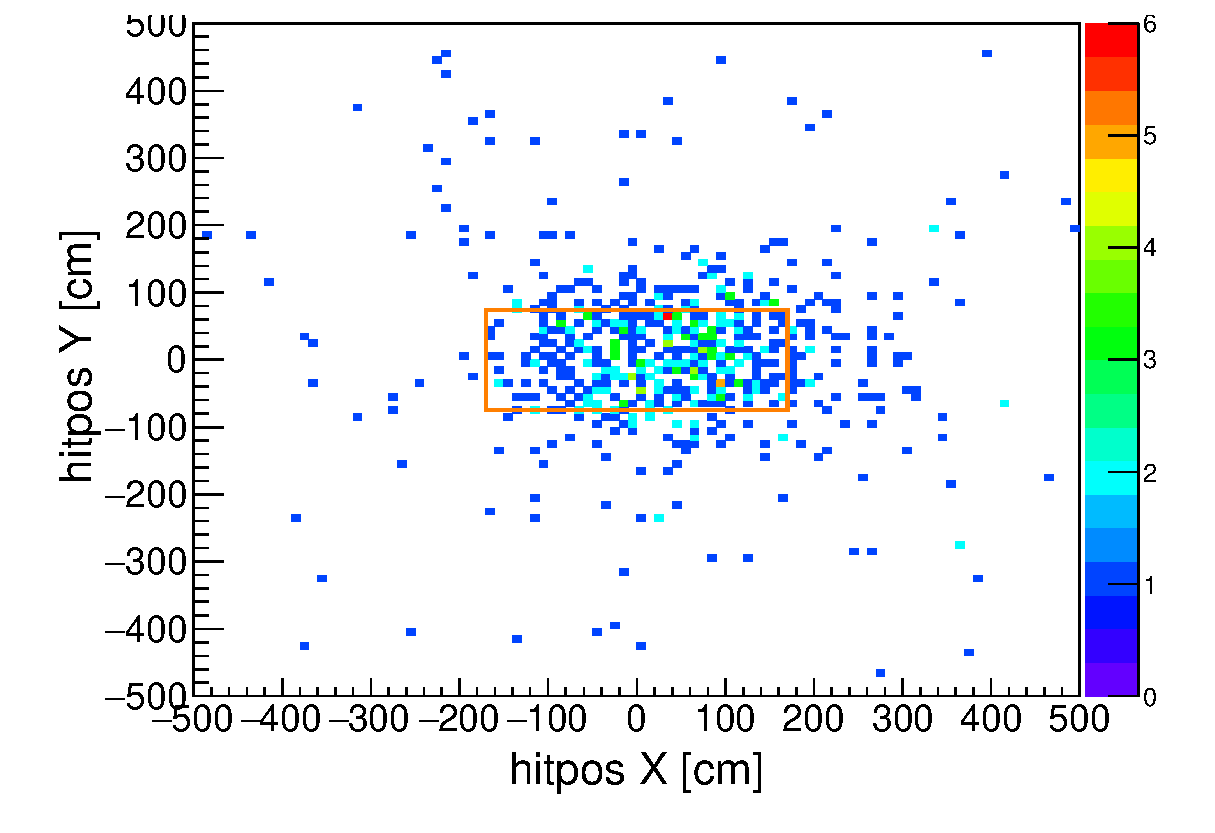
\includegraphics[width=5cm]{../pic/Run78/CDS_Lpim//kp_hitpos_Lpim_p_wHit.eps}
    \end{minipage}    
  \end{tabular}
  \caption{
    These figures show forward proton passing position calculated at the CVC.
    Right figure shows all events and left figure shows with events fired CVC or PC.
  }
  
  \label{fig:p_angle}
\end{figure}

The efficiency of the proton was scatted to forward angle was estimated using MR-RUN78.
The emmitted proton was defined by the CDS as Sec.\ref{sec:KP_timeoffset}.
In this purpose, sample events must be unbaised, so we used unbasied CDH3 trigger events as events samples.
The emmittion angle can be calculated from the masured particles as Fig.\ref{fig:p_angle}.
Because the proton scattered forward angle was bended by the Ushiwaka magnet, the efficiency of the proton maybe depends on the momentum of this.
Therefor, in our interest region, that seemsed almost flat value
that was guranteed by the MC sim and this effect convolved to the solid angle of the forward detectors, which discribed at Sec.\ref{sec:FC_SA}.\\
Fig\ref{fig:PCCVC_eff} indicates the relation of the selection region at CVC and the efficiency of forward detectors.
The selection region was estimated calculated hit position of z position at CVC using a straight line.
The selection region was not considered bending angle deu to the Ushiwaka, becaouse the effect was evaluated using the MC sim which was described Sec\ref{sec:sim_FC}.
The efficiency was saturated at the position is $-30$ cm, so we evaluated the efficiency was $0.819 \pm 0.042$.

\begin{figure}[htbp]
  \centering
  \begin{tabular}{cc}
    \begin{minipage}{0.5\hsize}
      \includegraphics[width=5cm]{../pic/Run78/KP_ana/Lpim_IM_hitpos_5.eps}
    \end{minipage}

    \begin{minipage}{0.5\hsize}
      \includegraphics[width=5cm]{../pic/Run78/KP_ana/Lpim_IM_hitpos_5_1350_1900.eps}
    \end{minipage}    
  \end{tabular}

  \caption{
    These figures shows invariant mass of $\Lambda$ $\pi^-$ that is cut by the size of counter is $-30$ cm.
    Left figure indicates around the region of interest and right figure indicates whole regtion.
    Black line indicates no selection and red line indicates with PC or CVC is fired events.
    Efficiency seems to be drastically dropped from 1.7 $GeV/c^2$.
  }
  
  \label{fig:IM_Lpim}
\end{figure}

\begin{figure}[htbp]
  \centering
  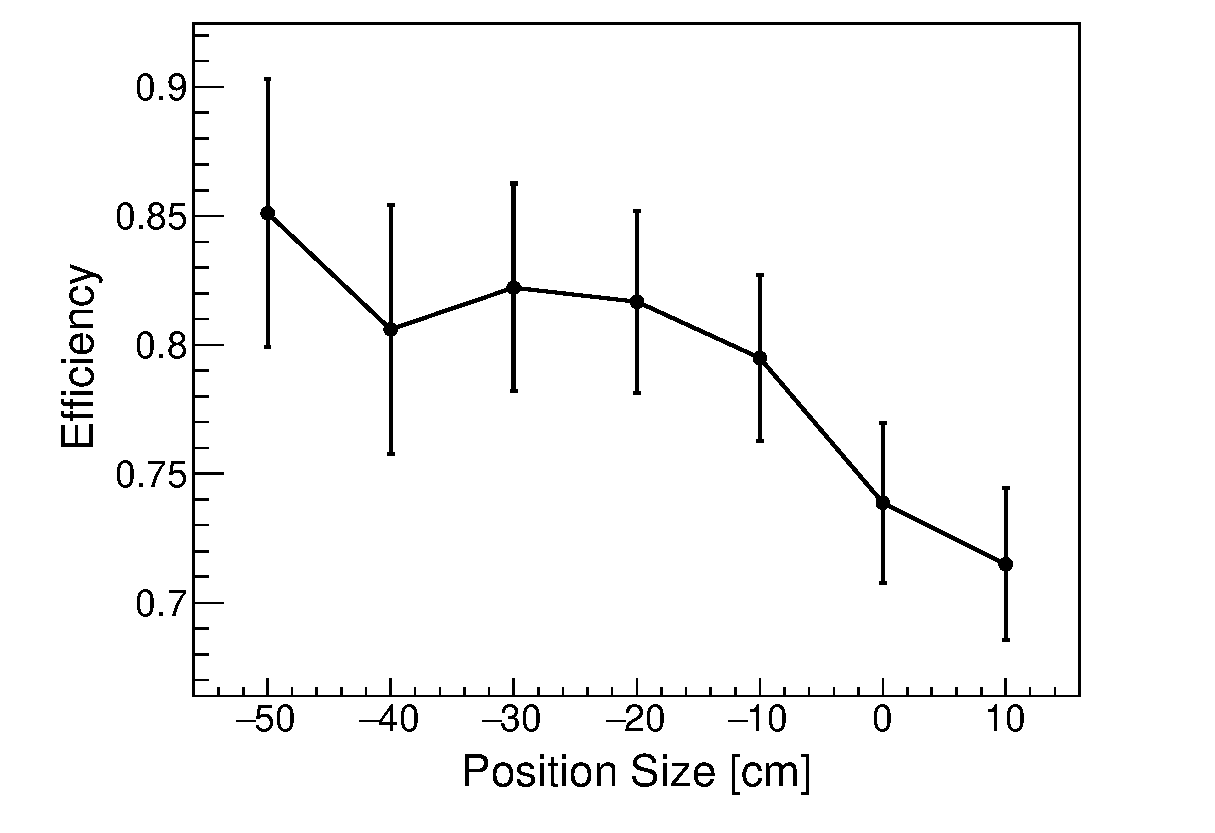
\includegraphics[width=8cm]{../pic/Run78/KP_ana/PCCVC_eff.eps}
  \caption{
    This figure shows the efficiency of forward detectors in each selection region at the CVC position.
    Error bars indicate statical error for the number of events.
  }
  \label{fig:PCCVC_eff}
\end{figure}





